\documentclass{standalone}
\usepackage{pgfplots, tikz}
	\pgfplotsset{compat=1.13}				
		   \usetikzlibrary{arrows.meta}

\begin{document}
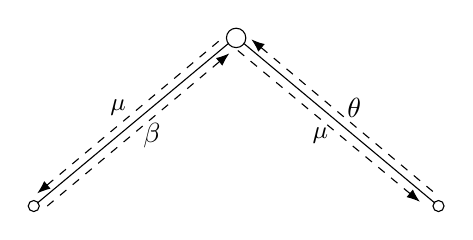
\begin{tikzpicture}
	\begin{axis}[
	xmin=-2,xmax=14,
	ymin=-2,ymax=14,
	grid=both,
	grid style={line width=.1pt, draw=darkgray!10},
	major grid style={line width=.2pt,draw=darkgray!50},
	axis lines=none,
	minor tick num=4,
	axis line style={-latex},	
	xlabel=$x$,	ylabel=$y$,
	]
	\draw[] (12,0) circle (2pt);
	\draw[] (0,0) circle (2pt);
	\draw[] (6,6) circle (3.5pt);
	\draw (0.1,0.1) -- (5.77,5.8);
	\draw (6.23,5.8) -- (11.9,0.1);
	\draw[Latex-, dashed] (0.1,0.45) -- (5.6,6);
	\draw[-Latex, dashed] (0.4,0) -- (5.8,5.45);
	\draw[Latex-, dashed] (6.45,5.95) -- (12,0.35);
	\draw[-Latex, dashed] (6.05,5.55) -- (11.45,0.15);
	\node at (2.5,3.5) {\small$\mu$};
	\node at (8.5,2.5) {\small$\mu$};
	\node at (3.5,2.5) {$\beta$};
	\node at (9.5,3.5) {$\theta$};
	\end{axis}
\end{tikzpicture}
\end{document}